%%%%%%%%%%%%%%%%%%%%%%%%%%%%%%%%%%%%%%%%%
% Beamer Presentation
% LaTeX Template
% Version 1.0 (10/11/12)
%
% This template has been downloaded from:
% http://www.LaTeXTemplates.com
%
% License:
% CC BY-NC-SA 3.0 (http://creativecommons.org/licenses/by-nc-sa/3.0/)
%
%%%%%%%%%%%%%%%%%%%%%%%%%%%%%%%%%%%%%%%%%

%----------------------------------------------------------------------------------------
%	PACKAGES AND THEMES
%----------------------------------------------------------------------------------------

\documentclass{beamer}

\mode<presentation> {

% The Beamer class comes with a number of default slide themes
% which change the colors and layouts of slides. Below this is a list
% of all the themes, uncomment each in turn to see what they look like.

%\usetheme{default}
%\usetheme{AnnArbor}
%\usetheme{Antibes}
%\usetheme{Bergen}
%\usetheme{Berkeley}
%\usetheme{Berlin}
%\usetheme{Boadilla}
%\usetheme{CambridgeUS}
%\usetheme{Copenhagen}
%\usetheme{Darmstadt}
%\usetheme{Dresden}
%\usetheme{Frankfurt}
%\usetheme{Goettingen}
%\usetheme{Hannover}
%\usetheme{Ilmenau}
%\usetheme{JuanLesPins}
%\usetheme{Luebeck}
\usetheme{Madrid}
%\usetheme{Malmoe}
%\usetheme{Marburg}
%\usetheme{Montpellier}
%\usetheme{PaloAlto}
%\usetheme{Pittsburgh}
%\usetheme{Rochester}
%\usetheme{Singapore}
%\usetheme{Szeged}
%\usetheme{Warsaw}

% As well as themes, the Beamer class has a number of color themes
% for any slide theme. Uncomment each of these in turn to see how it
% changes the colors of your current slide theme.

%\usecolortheme{albatross}
%\usecolortheme{beaver}
%\usecolortheme{beetle}
%\usecolortheme{crane}
%\usecolortheme{dolphin}
%\usecolortheme{dove}
%\usecolortheme{fly}
%\usecolortheme{lily}
%\usecolortheme{orchid}
%\usecolortheme{rose}
%\usecolortheme{seagull}
%\usecolortheme{seahorse}
%\usecolortheme{whale}
%\usecolortheme{wolverine}

\setbeamertemplate{footline} % To remove the footer line in all slides uncomment this line
%\setbeamertemplate{footline}[page number] % To replace the footer line in all slides with a simple slide count uncomment this line

\setbeamertemplate{navigation symbols}{} % To remove the navigation symbols from the bottom of all slides uncomment this line
}

\usepackage[all]{xy}  % Tool for drawing commutative diagrams
%\usepackage{tikz}     % A tool for drawing
\usepackage{graphicx} % Allows including images
\usepackage{booktabs} % Allows the use of \toprule, \midrule and \bottomrule in tables

%----------------------------------------------------------------------------------------
%	TITLE PAGE
%----------------------------------------------------------------------------------------

\title[de Rham cohomology of hyperelliptic curves]{Group actions on the algebraic de Rham cohomology of hyperelliptic curves} % The short title appears at the bottom of every slide, the full title is only on the title page

\author{Joe Tait} % Your name
\institute[Southampton University] % Your institution as it will appear on the bottom of every slide, may be shorthand to save space
{
The University of Southampton   \\ % Your institution for the title page
\medskip
\textit{joe.tait@soton.ac.uk} % Your email address
}
\date{\today} % Date, can be changed to a custom date

\begin{document}


%\begin{frame}
%\end{frame}
%
%%----------------------------------------------------------------------------------------
%%	PRESENTATION SLIDES
%%----------------------------------------------------------------------------------------
%
%%------------------------------------------------
%\section{First Section} % Sections can be created in order to organize your presentation into discrete blocks, all sections and subsections are automatically printed in the table of contents as an overview of the talk
%%------------------------------------------------
%
%\subsection{Subsection Example} % A subsection can be created just before a set of slides with a common theme to further break down your presentation into chunks
%
%\begin{frame}
%\frametitle{Paragraphs of Text}
%Sed iaculis dapibus gravida. Morbi sed tortor erat, nec interdum arcu. Sed id lorem lectus. Quisque viverra augue id sem ornare non aliquam nibh tristique. Aenean in ligula nisl. Nulla sed tellus ipsum. Donec vestibulum ligula non lorem vulputate fermentum accumsan neque mollis.\\~\\
%
%Sed diam enim, sagittis nec condimentum sit amet, ullamcorper sit amet libero. Aliquam vel dui orci, a porta odio. Nullam id suscipit ipsum. Aenean lobortis commodo sem, ut commodo leo gravida vitae. Pellentesque vehicula ante iaculis arcu pretium rutrum eget sit amet purus. Integer ornare nulla quis neque ultrices lobortis. Vestibulum ultrices tincidunt libero, quis commodo erat ullamcorper id.
%\end{frame}
%
%%------------------------------------------------
%
%\begin{frame}
%\frametitle{Bullet Points}
%\begin{itemize}
%\item Lorem ipsum dolor sit amet, consectetur adipiscing elit
%\item Aliquam blandit faucibus nisi, sit amet dapibus enim tempus eu
%\item Nulla commodo, erat quis gravida posuere, elit lacus lobortis est, quis porttitor odio mauris at libero
%\item Nam cursus est eget velit posuere pellentesque
%\item Vestibulum faucibus velit a augue condimentum quis convallis nulla gravida
%\end{itemize}
%\end{frame}
%
%%------------------------------------------------
%
%\begin{frame}
%\frametitle{Blocks of Highlighted Text}
%\begin{block}{Block 1}
%Lorem ipsum dolor sit amet, consectetur adipiscing elit. Integer lectus nisl, ultricies in feugiat rutrum, porttitor sit amet augue. Aliquam ut tortor mauris. Sed volutpat ante purus, quis accumsan dolor.
%\end{block}
%
%\begin{block}{Block 2}
%Pellentesque sed tellus purus. Class aptent taciti sociosqu ad litora torquent per conubia nostra, per inceptos himenaeos. Vestibulum quis magna at risus dictum tempor eu vitae velit.
%\end{block}
%
%\begin{block}{Block 3}
%Suspendisse tincidunt sagittis gravida. Curabitur condimentum, enim sed venenatis rutrum, ipsum neque consectetur orci, sed blandit justo nisi ac lacus.
%\end{block}
%\end{frame}
%
%%------------------------------------------------
%
%\begin{frame}
%\frametitle{Multiple Columns}
%\begin{columns}[c] % The "c" option specifies centered vertical alignment while the "t" option is used for top vertical alignment
%
%\column{.45\textwidth} % Left column and width
%\textbf{Heading}
%\begin{enumerate}
%\item Statement
%\item Explanation
%\item Example
%\end{enumerate}
%
%\column{.5\textwidth} % Right column and width
%Lorem ipsum dolor sit amet, consectetur adipiscing elit. Integer lectus nisl, ultricies in feugiat rutrum, porttitor sit amet augue. Aliquam ut tortor mauris. Sed volutpat ante purus, quis accumsan dolor.
%
%\end{columns}
%\end{frame}
%
%%------------------------------------------------
%\section{Second Section}
%%------------------------------------------------
%
%\begin{frame}
%\frametitle{Table}
%\begin{table}
%\begin{tabular}{l l l}
%\toprule
%\textbf{Treatments} & \textbf{Response 1} & \textbf{Response 2}\\
%\midrule
%Treatment 1 & 0.0003262 & 0.562 \\
%Treatment 2 & 0.0015681 & 0.910 \\
%Treatment 3 & 0.0009271 & 0.296 \\
%\bottomrule
%\end{tabular}
%\caption{Table caption}
%\end{table}
%\end{frame}
%
%%------------------------------------------------
%
%\begin{frame}
%\frametitle{Theorem}
%\begin{theorem}[Mass--energy equivalence]
%$E = mc^2$
%\end{theorem}
%\end{frame}
%
%%------------------------------------------------
%
%\begin{frame}[fragile] % Need to use the fragile option when verbatim is used in the slide
%\frametitle{Verbatim}
%\begin{example}[Theorem Slide Code]
%\begin{verbatim}
%\begin{frame}
%\frametitle{Theorem}
%\begin{theorem}[Mass--energy equivalence]
%$E = mc^2$
%\end{theorem}
%\end{frame}\end{verbatim}
%\end{example}
%\end{frame}
%
%%------------------------------------------------
%

\begin{frame}
\only<1>{\begin{displaymath}
    \xymatrix{
    0 \ar[r] & \Omega^0_X \ar@[white][d] \ar[r] & \Omega_X^1 \ar[r] \ar@[white][d] & \ldots \ar[r] & \Omega_X^n \ar@[white][d] \ar[r] & 0 \\ 
    {\color{white}0 \ar@[white][r]} & {\color{white}C^0(\Omega^0_X) \ar@[white][d] \ar@[white][r] } & {\color{white}C^0(\Omega_X^1) \ar@[white][r] \ar@[white][d] } & {\color{white}\ldots \ar@[white][r] } & {\color{white}C^0(\Omega_X^n) \ar@[white][d] \ar@[white][r] } & {\color{white}0} \\
    {\color{white}0 \ar@[white][r]} & {\color{white}C^1(\Omega^0_X) \ar@[white][d] \ar@[white][r] } & {\color{white}C^1(\Omega_X^1) \ar@[white][r] \ar@[white][d] } & {\color{white}\ldots \ar@[white][r] } & {\color{white}C^1(\Omega_X^n) \ar@[white][d] \ar@[white][r] } & {\color{white}0} \\
    &   {\color{white} \vdots}                       & {\color{white}\vdots                        } & {\color{white}\ldots        } & {\color{white}\vdots                        } &  \\
    }
\end{displaymath}}

\only<2>{\begin{displaymath}
    \xymatrix{
    0 \ar[r] & \Omega^0_X \ar[d] \ar[r] & \Omega_X^1 \ar[r] \ar@[white][d] & \ldots \ar[r] & \Omega_X^n \ar@[white][d] \ar[r] & 0 \\ 
    {\color{white}0 \ar@[white][r]} & C^0(\Omega^0_X) \ar[d] \ar@[white][r]  & {\color{white}C^0(\Omega_X^1) \ar@[white][r] \ar@[white][d] } & {\color{white}\ldots \ar@[white][r] } & {\color{white}C^0(\Omega_X^n) \ar@[white][d] \ar@[white][r] } & {\color{white}0} \\
    {\color{white}0 \ar@[white][r]} & C^1(\Omega^0_X) \ar[d] \ar@[white][r]  & {\color{white}C^1(\Omega_X^1) \ar@[white][r] \ar@[white][d] } & {\color{white}\ldots \ar@[white][r] } & {\color{white}C^1(\Omega_X^n) \ar@[white][d] \ar@[white][r] } & {\color{white}0} \\
    &    \vdots                       & {\color{white}\vdots                        } & {\color{white}\ldots        } & {\color{white}\vdots                        } &  \\
    }
\end{displaymath}}

\only<3>{\begin{displaymath}
    \xymatrix{
    0 \ar[r] & \Omega^0_X \ar[d] \ar[r] & \Omega_X^1 \ar[r] \ar[d] & \ldots \ar[r] & \Omega_X^n \ar[d] \ar[r] & 0 \\ 
    0 \ar[r] & C^0(\Omega^0_X) \ar[d] \ar[r] & C^0(\Omega_X^1) \ar[r] \ar[d] & \ldots \ar[r] & C^0(\Omega_X^n) \ar[d] \ar[r] & 0 \\
    0 \ar[r] & C^1(\Omega^0_X) \ar[d] \ar[r] & C^1(\Omega_X^1) \ar[r] \ar[d] & \ldots \ar[r] & C^1(\Omega_X^n) \ar[d] \ar[r] & 0 \\
    &   \vdots                       & \vdots                        & \ldots        & \vdots                        & \\
    }
\end{displaymath}}

\only<4>{\begin{displaymath}
    \xymatrix{
    0 \ar[r] & {\color{red}\Omega^0_X} \ar[d] \ar[r] & \Omega_X^1 \ar[r] \ar[d] & \ldots \ar[r] & \Omega_X^n \ar[d] \ar[r] & 0 \\ 
    0 \ar[r] & C^0(\Omega^0_X) \ar[d] \ar[r] & C^0(\Omega_X^1) \ar[r] \ar[d] & \ldots \ar[r] & C^0(\Omega_X^n) \ar[d] \ar[r] & 0 \\
    0 \ar[r] & C^1(\Omega^0_X) \ar[d] \ar[r] & C^1(\Omega_X^1) \ar[r] \ar[d] & \ldots \ar[r] & C^1(\Omega_X^n) \ar[d] \ar[r] & 0 \\
    &   \vdots                       & \vdots                        & \ldots        & \vdots                        & \\
    }
\end{displaymath}

\begin{displaymath}
\xymatrix{
0 \ar[r]  & \Omega_X^0 \ar@[white][r] & {\color{white} C^0(\Omega_X^0) \oplus \Omega_X^1 } \ar@[white][r] & {\color{white} C^1(\Omega_X^0) \oplus C^0(\Omega_X^1) \oplus \Omega_X^2} \ar@[white][r] &
}
\end{displaymath}}


\only<5>{\begin{displaymath}
    \xymatrix{
    0 \ar[r] & \Omega^0_X \ar[d] \ar[r] & {\color{red}\Omega_X^1} \ar[r] \ar[d] & \ldots \ar[r] & \Omega_X^n \ar[d] \ar[r] & 0 \\ 
    0 \ar[r] & {\color{red}C^0(\Omega^0_X)} \ar[d] \ar[r] & C^0(\Omega_X^1) \ar[r] \ar[d] & \ldots \ar[r] & C^0(\Omega_X^n) \ar[d] \ar[r] & 0 \\
    0 \ar[r] & C^1(\Omega^0_X) \ar[d] \ar[r] & C^1(\Omega_X^1) \ar[r] \ar[d] & \ldots \ar[r] & C^1(\Omega_X^n) \ar[d] \ar[r] & 0 \\
    &   \vdots                       & \vdots                        & \ldots        & \vdots                        & \\
    }
\end{displaymath}

\begin{displaymath}
\xymatrix{
0 \ar[r]  & \Omega_X^0 \ar[r] & C^0(\Omega_X^0) \oplus \Omega_X^1  \ar@[white][r] & {\color{white} C^1(\Omega_X^0) \oplus C^0(\Omega_X^1) \oplus \Omega_X^2} \ar@[white][r] &
}
\end{displaymath}}

\only<6>{\begin{displaymath}
    \xymatrix{
    0 \ar[r] & \Omega^0_X \ar[d] \ar[r] & \Omega_X^1 \ar[r] \ar[d] & \ldots \ar[r] & \Omega_X^n \ar[d] \ar[r] & 0 \\ 
    0 \ar[r] & C^0(\Omega^0_X) \ar[d] \ar[r] & {\color{red}C^0(\Omega_X^1)} \ar[r] \ar[d] & \ldots \ar[r] & C^0(\Omega_X^n) \ar[d] \ar[r] & 0 \\
    0 \ar[r] & {\color{red}C^1(\Omega^0_X)} \ar[d] \ar[r] & C^1(\Omega_X^1) \ar[r] \ar[d] & \ldots \ar[r] & C^1(\Omega_X^n) \ar[d] \ar[r] & 0 \\
    &   \vdots                       & \vdots                        & \ldots        & \vdots                        & \\
    }
\end{displaymath}

\begin{displaymath}
\xymatrix{
0 \ar[r]  & \Omega_X^0 \ar[r] & C^0(\Omega_X^0) \oplus \Omega_X^1  \ar[r] & C^1(\Omega_X^0) \oplus C^0(\Omega_X^1) \oplus \Omega_X^2 & 
}
\end{displaymath}}
\end{frame}

%\begin{frame}
%\frametitle{Hyperelliptic curve}
%\begin{figure}
%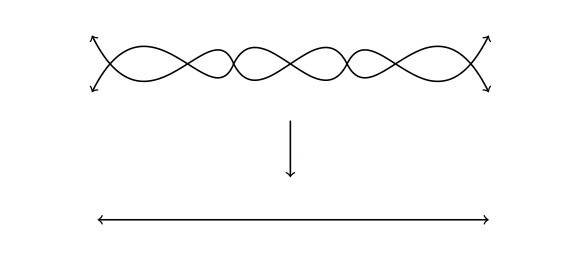
\includegraphics[width=0.8\linewidth]{Double_Cover.jpg}
%\end{figure}
%\end{frame}
%
\begin{frame}
\frametitle{$\check{\text C}$ech complex}
The $\check {\text C}$ech complex of $X$ with respect to this cover is
\[
\begin{array}{ccc}
        O_X(U_0)\times O_X(U_\infty) & \xrightarrow^{d \times d}  & \Omega^1_X(U_0) \times \Omega_X^1(U_\infty)  \\
        \downarrow \check{d}             &           & \downarrow \check{d}\\
        O_X(U_0\cap U_\infty) & \xrightarrow^{d}                      & \Omega_X^1(U_0 \cap U_\infty)
\end{array}
\]
\pause

which gives rise to the following total complex
\begin{equation*}
O_X(U_0) \times O_X(U_\infty) \xrightarrow^{d_0} \Omega_X^1(U_0)\times \Omega_X^1(U_\infty) \times O_X(U_0 \cap U_\infty) \xrightarrow^{d_1} \Omega^1_X(U_0 \cap U_\infty).
\end{equation*}
\pause
Then $H^1_{\text dR}(X) \cong \check{H}^1_{\text dR}(U) = \operatorname{ker}(d_1)/\operatorname{im}(d_0)$, which has elements of the form $(f_0, f_\infty , \omega)$.
\end{frame}

\begin{frame}
For each $1\leq i \leq g$, $1\le j \leq 2g+2$ and $0\leq k \leq g+1$ we choose $A_{i,j}$ and $B_{i,k}$ in $k$ such that if we let
\[
\Phi_i(x,y) = A_{i,2g+2}x^{2g+2} + \ldots + A_{i,i+1}x^{i+1} + y(B_{i,g}x^g + \ldots + B_{i,i+1}x^{i+1})
\]
and
\[
\Psi_i(x,y) = A_{i,i}x^{i} + \ldots + A_{i,1}x+ y(B_{i,i-1}x^{i-1} + \ldots + B_{i,1}x B_{i,0}).
\]
then
\[
xF'(x) + y(xH'(x) + iH(x)) = \Phi_i(x,y) + \Psi_i(x,y).
\]
\pause
\begin{theorem}
The residue classes of
\[
\tau_i := \left( \left( \frac{\Psi_i(x,y)}{x^{i+1}H(x)} \right) \only<1>{dx}, \left(\frac{-\Phi_i(x)}{x^{i+1}H(x)} \right)dx, \frac{y}{x^i} \right), i= 1, \ldots, g
\]
and
\[
\nu_i := \left( \frac{x^i}{H(x)}dx, \frac{x^i}{H(x)}dx, 0 \right), i = 0, \ldots, g-1
\]
form a $k$-basis of $\check{H}^1_X(U)$.

\end{theorem}
\end{frame}

\begin{frame}
For each $i \in \{1, \ldots, g\}, k \in \{0, \ldots , 2g+2\}$ we define $\alpha_{i,k}\in k$ such that
\[
xf'(x) - 2if(x) = \alpha_{i,2g+2}x^{2g+2} + \alpha_{i, 2g+1}x^{2g+2} + \ldots + \alpha_{i,0}
\]
and then define
\[
\phi_i(x)  := \alpha_{i,2g+2}x^{2g+2} + \ldots + \alpha_{i,g+2}x^{g+2} 
\]
and
\[
\psi_i(x) := \alpha_{i,g+1}x^{g+1} + \ldots + \alpha_{i,0}.
\]
\pause
\begin{theorem}
The residue classes of
\[
\tau_i := \left( \left( \frac{\psi_i(x)}{2yx^{i+1}} \right) \only<1>{dx}, \left(\frac{-\phi_i(x)}{2yx^{i+1}} \right)dx, \frac{y}{x^i} \right), i= 1, \ldots, g
\]
and
\[
\nu_i := \left( \frac{x^i}{y}dx, \frac{x^i}{y}dx, 0 \right), i = 0, \ldots, g-1
\]
form a $k$-basis of $\check{H}^1_X(U)$.
\end{theorem}
\end{frame}

\begin{frame}
We define 
\[
r_i(x) = \sum_{k=0}^{i-1} (-1)^{g-k} \binom{g}{k} a^{g-k}x^k \quad {\text and} \quad t_i(x) = \sum_{k=i}^g (-1)^{g-k}\binom{g}{k} a^{g-k}x^k.
\]
\begin{theorem}
The pre-image $\rho^{-1}(\tau_i)$ is the residue class of is
\begin{equation*}
\left( \frac{\psi_i(x)}{2yx^{i+1}}dx, \frac{h_i}{2yx^{i+1}(x-a)^{g+1}}dx, \frac{-\phi_i(x)}{2yx^{i+1}}dx, \frac{r_i(x)y}{x^i(x-a)^g}, \frac{y}{x^i}, \frac{t_i(x)y}{x^i(x-a)^g} \right)
\end{equation*}
where
\[
h_i = 
(\psi_i(x)t_i(x) - \phi_i(x)r_i(x))(x-a) + 2if(x)(-1)^{g-i+1}\binom{g}{i}a^{g-i+1}x^i.
\]
\end{theorem}

\end{frame}
%
%%------------------------------------------------
%
%\begin{frame}[fragile] % Need to use the fragile option when verbatim is used in the slide
%\frametitle{Citation}
%An example of the \verb|\cite| command to cite within the presentation:\\~
%
%This statement requires citation \cite{p1}.
%\end{frame}
%
%%------------------------------------------------
%
%\begin{frame}
%\frametitle{References}
%\footnotesize{
%\begin{thebibliography}{99} % Beamer does not support BibTeX so references must be inserted manually as below
%\bibitem[Smith, 2012]{p1} John Smith (2012)
%\newblock Title of the publication
%\newblock \emph{Journal Name} 12(3), 45 -- 678.
%\end{thebibliography}
%}
%\end{frame}
%
%%------------------------------------------------
%
%\begin{frame}
%\Huge{\centerline{The End}}
%\end{frame}
%
%----------------------------------------------------------------------------------------
\end{document} 
